\documentclass[manuscript,review,anonymous,authoryear]{acmart}

\citestyle{acmauthoryear}
\usepackage{graphicx}

\usepackage{xurl}

\usepackage{placeins}

\setcopyright{none}

\settopmatter{printacmref=false}

\renewcommand{\footnotetextcopyrightpermission}[1]{}

\acmYear{2027}

\acmSubmissionID{Pending}

\title{Re-developing Memory}

\subtitle{Narrative-Driven Photographic Re-creation and the Boundaries of Recording Memory Images}

\begin{document}

\begin{abstract}

Does a photograph have only one final form? Digital photography transforms sensor data through an imaging pipeline into determinate color, brightness, and sharpness. Sampling structures, calibration differences, and unused rendering outcomes are seldom made available for viewing. Taking this as a starting point, this study presents Re-developing Memory: participants upload personal photographs and write recollections; a system selects image operations through semantic analysis and combines variations re-derived from RAW data, non-generative operations drawn from photographic art, and provenance-marked local generation. One photograph thereby acquires multiple possible forms through successive stages. Each cumulative stage is saved, and corresponding vertical strips are finally juxtaposed into one memory image. The study refers philosophically to Bergson's notion of virtual memory and situates its practice in contemporary photography's use of defocus, concealment, and digital imperfections. Rather than recovering a uniquely true memory, the work uses contemporary AI and photographic processing to propose a form of 'photographic poetry' whose formation remains visible.

\end{abstract}

\keywords{photographic poetry; RAW; image signal processing; re-development; personal memory; generative imagery; medium specificity}

\maketitle

\section{Introduction: How a Photograph Becomes Final}

When the shutter is pressed, a camera follows a predefined imaging process: sensor data still undergo white balance, demosaicing, denoising, color conversion, tone mapping, and other operations before optical information becomes a viewable photograph. The final color and sharpness are engineering output choices, but also embody conventions of 'correct' viewing. Images not selected within this process, suppressed noise, unreconstructed colors, and brightness relations under alternative parameters are obscured within the imaging space. Could these data nevertheless contain a kind of poetry?


Personal recollection does not follow the fixed boundaries of a photograph either. A clear photograph may correspond to a blurred memory; an object frozen by the shutter may remain in motion in recollection; a gesture excluded from the frame may become the most important part of remembering.


In this system, I am not concerned with turning a photograph into a spatially correct image that strictly respects the instant the shutter was pressed. Instead, I invite recollection back into the formation of the photograph: could states formerly regarded as technical defects, together with artistic procedures of concealment, cutting, and duplication, become other forms of that photograph?


Accordingly, the artwork uses an image system driven jointly by an original photograph and text: it analyzes recollection, proposes operations, alters the image step by step, preserves intermediate stages, and finally assembles different moments into a single work. This paper examines three questions: (1) how recollections can be translated into image operations with global or local scopes; (2) how the camera pipeline offers a technical point of reference for photography's unfinishedness, and how contemporary photographic forms can become a poetic language responsive to memory; and (3) how traceable provenance boundaries can be maintained between conjecture and newly added content introduced by AI generation.


\section{Theoretical, Technical, and Artistic Context}

\subsection{The Imaging Pipeline and Multiple Possible Forms of Photography}

In a typical Bayer color filter array, RGGB denotes the arrangement of color sampling sites; a single site generally does not record complete RGB information. Demosaicing reconstructs color, while black-level correction, noise reduction (NR), white balance (WB), color correction matrices (CCM), tone mapping, and gamma encoding participate in the formation of a photograph. Some pipelines also use Y$\prime$CbCr (often loosely called YUV) to process luma and chroma channels. The order and algorithms vary among cameras, and not every stage corresponds to a complete, directly viewable image.


Not every ISP stage corresponds to a complete photograph ready to be viewed. Yet these technical processes show that a photograph's final appearance depends on a series of selectable treatments. The same capture data can yield different results through white balance, tone curves, or denoising strategies. Flusser's (2000 [1983]) discussion of the photographic apparatus and its program offers a media-theoretical perspective: photography involves not only framing and releasing the shutter, but also the organization of possibilities preset by equipment. This work makes such normally hidden programmatic choices objects of viewing: noise may remain, color may deviate, an image may lose focus, and a corrected-away state may become part of the artwork.


\subsection{Bergson: The Virtuality and Actualization of Memory}

In Matter and Memory, Bergson distinguishes virtual recollection from the concrete form it acquires in the present, discussing how memory gradually becomes actualized and approaches perception (Bergson 1991 [1896]). The past persists virtually and takes on a concrete form through the present activity of recollection.


A recollection is not a perfect photographic original. When the same experience is recalled at different times, certain details may emerge while others recede into an indistinct background.


This virtuality inspires the work, but it is not identical to intermediate ISP data. The former concerns philosophical questions of time, consciousness, and the existence of the past; the latter is a technically describable processing sequence. I use the photographic process to develop a viewable artistic form for the way 'memory takes shape again in the present.'


\subsection{From the Photographic Medium to ``Photographic Poetry''}

In a text on 'Plastic Poetry' published in VOU in 1966, Kitasono Katue proposed composing poetry with cameras and images, without reliance on conventional lines of verse. In this sense, 'photographic poetry' is not merely a lyrical text accompanying a photograph: images, selection, sequence, editing, damage, intervals, and material form can themselves produce poetry (Kitasono 1966; Mayer 1971).


Contemporary photography has likewise transformed 'incompleteness' into form. Andreas Müller-Pohle's Digital Scores (1995--1998) transcribes an early photograph into digital codes not directly legible to the human eye, making information itself a problem of viewing. Daido Moriyama and the vocabulary of are, bure, boke (graininess, movement, and defocus) show that grain and blur need not remain defects to be removed. Thomas Ruff's jpegs makes compression, pixel structure, and their visible traces part of the work's organization. These are not technical experiments in camera ISP, but they suggest how imperfections of a medium may become an aesthetic vocabulary.


Another thread involves disappearance and manual intervention. In Punched Out Stars (2011), Aspen Mays physically perforated photographs to remove stars; in Reconstruction of a Family (2016), Lebohang Kganye uses family photographs to produce silhouettes and scenes in which absence acquires a new material form. In this work, whitening, silhouette, overlay, slicing, and seams cannot be mere entries in an 'effects library': they should respond to what is seen, forgotten, touched, or left uncertain in the narrative.


Generated imagery raises a further boundary. Maria Mavropoulou's Imagined Images (2021--2023) generates a missing family album from inherited narratives; ReCollection (Zhang et al. 2024) uses language input to form synthetic memories. Unlike generation from scratch, this work always begins with an existing photograph, introduces generation only when the narrative points explicitly beyond the photographed content, and keeps conjecture identifiable as conjecture.


\section{Artistic Method: Layers of RAW, Photographic Operations, and Generation}

\subsection{Photograph and Recollection Jointly Specify Operations}

Participants upload RAW, JPEG, PNG, or other photographs they have taken and describe their memories of the scene or their feelings upon revisiting it. A vision-language model first identifies scenes, objects, and lighting; a language model then proposes the source phrase, target region, operation, and parameters. For local changes, masks are established using segmentation results such as those from SAM 2.1. The system validates the executable scope of operations, connecting natural language to traceable photographic processing.


\subsection{Making the Possibilities of Real RAW Pipelines Visible}

RAW becomes more than a file converted into a working image: sampling and repeated rendering become selectable material. With rawpy's raw\_image\_visible and raw\_colors\_visible, the uninterpolated color sampling may be displayed when Bayer RAW data are available. Changing demosaic\_algorithm or using half\_size produces different detail and interpolation outcomes. Separate renderings with user\_wb can produce different warmth and coolness; fbdd\_noise\_reduction, median\_filter\_passes, exp\_shift, and gamma involve alternative choices of noise reduction, brightness, and output curves. Such differences can answer phrases such as 'I remember only scattered colors,' 'the details are no longer clear,' or 'the light was colder then.'


The user\_black and user\_sat controls modify black level and saturation white level; they are not ordinary fading or saturation sliders. Raising part of an already exposed RAW image cannot retroactively recreate sensor saturation at capture. Uncorrected purple fringing or output in a RAW color space also does not guarantee a fixed aesthetic effect. If haze, local overexposure-like whitening, or stronger vignetting is required, the corresponding post-processing step should be identified. Here, 'real pipeline' therefore means a traceable RAW sampling or re-rendering branch; without the corresponding source data, the image can only simulate its visual language.


\subsection{Organizing Recollection Through Photographic Artistic Techniques}

The second group of operations adds no new objects; it reorganizes the visibility of what the photograph already contains. Defocus and synthesized depth of field redirect attention. Local whitening, negative images, silhouettes, color misregistration, and overlays express absence. Grain, scratches, pixel sorting, strip stretching, and fold-like seams expose the vulnerability of the image's surface. Blur derived from estimated depth is a synthetic effect, not a recovery of the original lens's depth of field. Fingerprints or touch traces added algorithmically must be recorded as procedural texture effects.


Operations are selected through 'verbs of recollection' rather than fixed style tags. 'Forget' may produce whitening or a silhouette that retains an outline; 'touch' may become an overlay or wiping gesture; 'uncertain' may take the form of shifting focus, chroma misregistration, or visible seams. The model offers interpretable candidates, while the image context and constrained rules determine where they act.


\subsection{Space Beyond the Photograph and Absent Things}

Only when a narrative explicitly requests content not present in the original photograph does the system employ local generation: for example, an unphotographed hand or a window outside the frame. Outpainting should likewise identify the original image boundary. Seamlessly removing an object and filling the background through generation is a different aesthetic decision from whitening the object while leaving an absent shape; the two should not both be called 'disappearance.'


\subsection{Cumulative Development and the Final Photographic Poem}

Operations are applied in interpreted order to the preceding image. Finally, borrowing the juxtaposition of darkroom test strips, the system extracts corresponding vertical strips from the original and successive stages and assembles them in one frame. It does not simply shrink multiple whole photographs into narrow pictures: different parts of the same spatial scene carry different moments of processing. The final form is a single photographic work.


\begin{figure}[htbp]

\centering

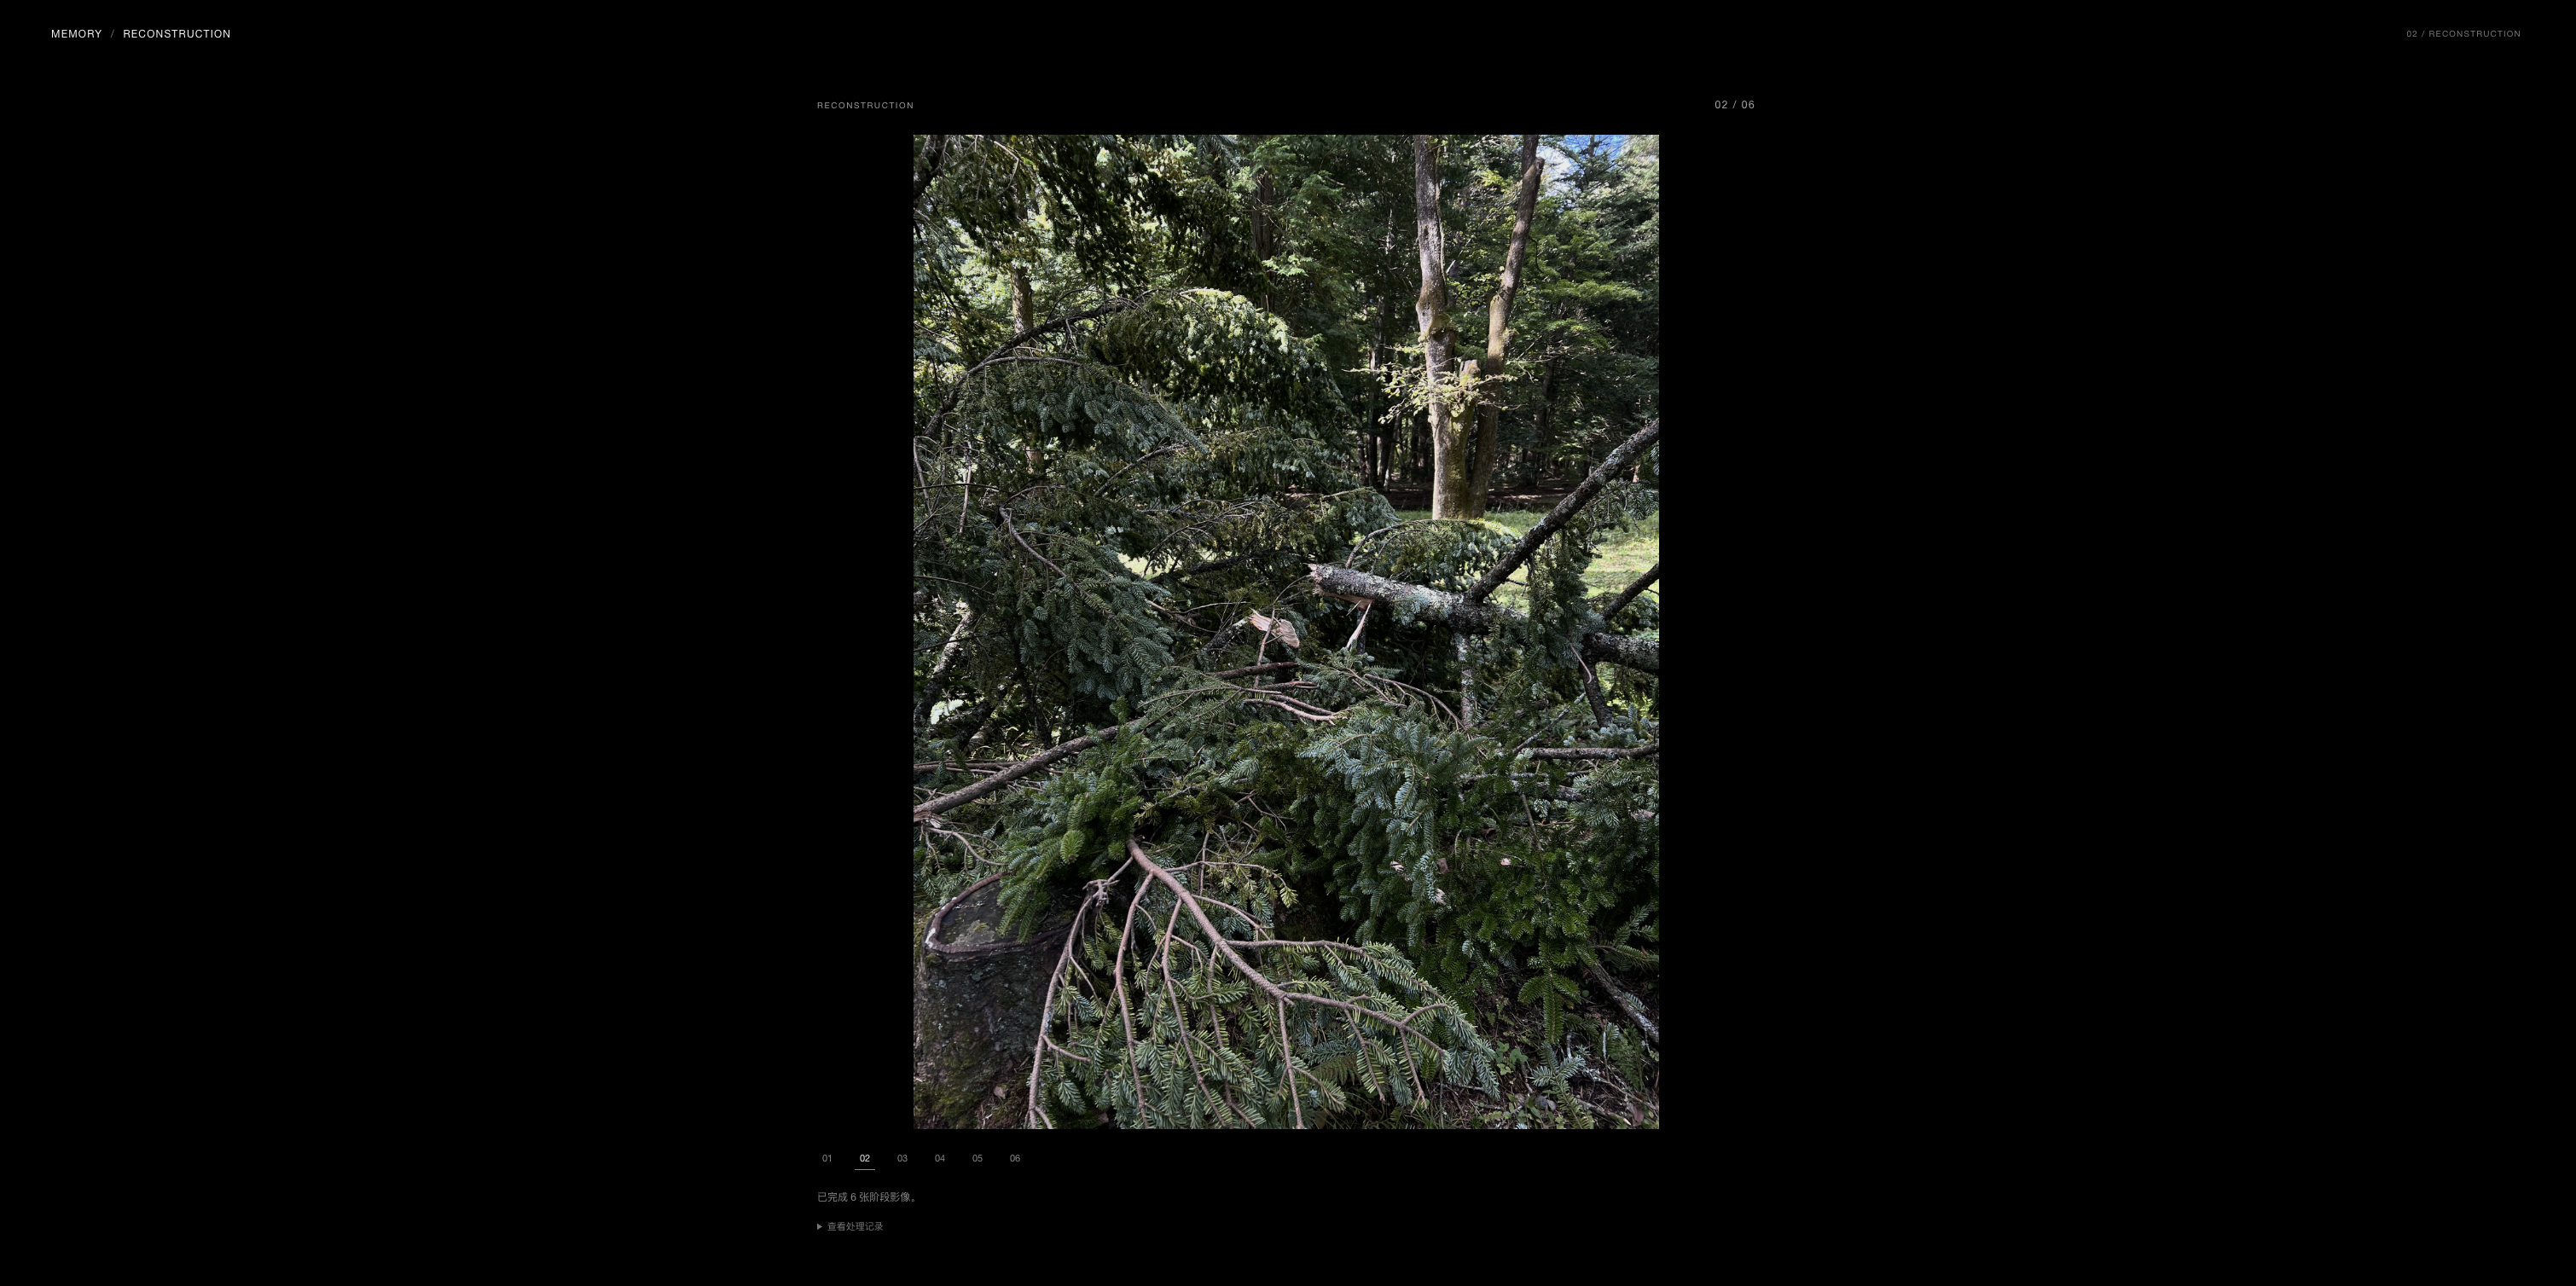
\includegraphics[width=.61\linewidth]{figures/ui_original_1.png}

\par\smallskip

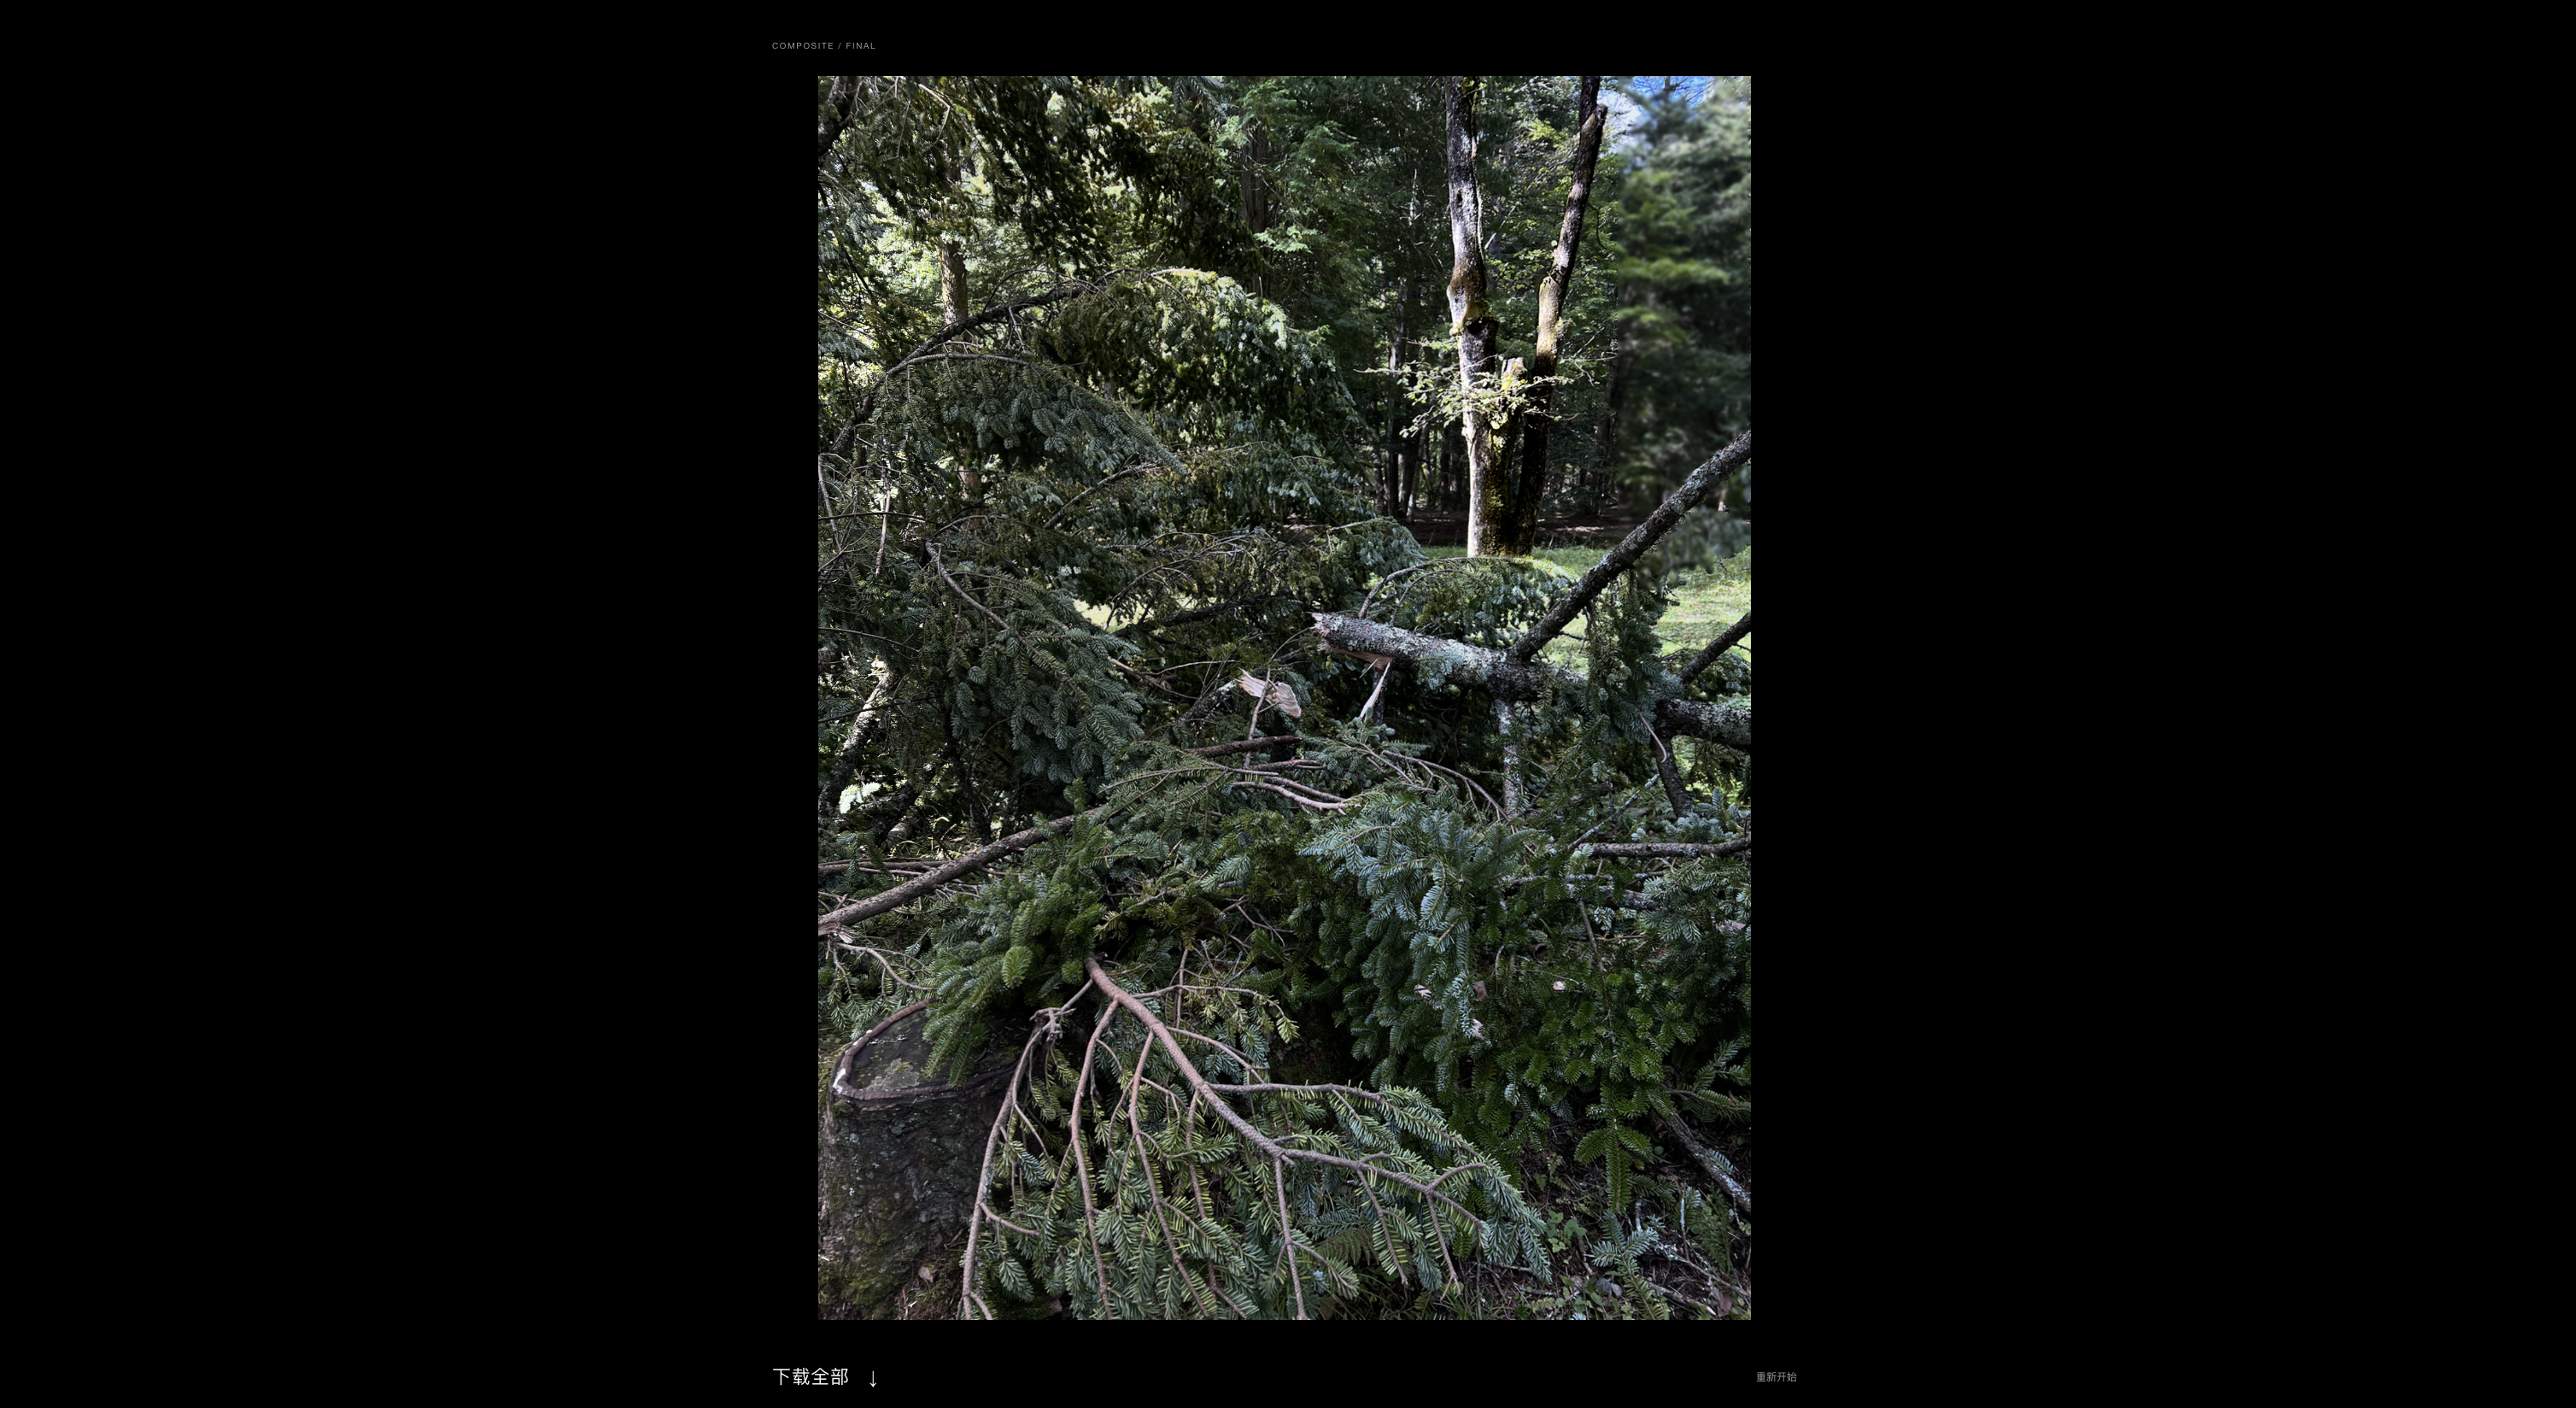
\includegraphics[width=.61\linewidth]{figures/ui_original_2.png}

\caption{Interface screenshots of Re-developing Memory: (a) the reconstruction screen shows a selected processing stage (02/06) and navigation between saved stages; (b) the final composite screen shows the assembled image and download control. Both panels reproduce full, uncropped screenshots of the working system interface.}

\Description{Two full uncropped system screenshots: the reconstruction stage viewer and the final composite display.}
\label{fig:interface}

\end{figure}

\FloatBarrier

\section{Artwork Case Studies}

\subsection{Pendulum: Time Within an Instant}

In the Foucault pendulum photograph, a metallic sphere hangs centrally above a circular numbered base, surrounded by a ring of lights and a dome. The participant wrote: 'I always felt it should have been darker overall; the bright areas were not that bright either. The pendulum sphere was moving, and the surrounding walls resemble a vignette. Perhaps add a vintage-looking vignette?' The saved execution log records four completed operations in sequence: global exposure $-$0.35 EV; local exposure of the light ring $-$0.42 EV; motion blur of the sphere (amount = 0.11; angle = 0$^\circ$); and vignetting (amount = 0.12). The direction is an algorithmic setting, not a measurement of the pendulum's actual motion.


The photograph fixes the pendulum in a single still instant, whereas the participant recalls continuous movement. A time-related blur allows the clear sphere to acquire the possibility of motion again. The case brings photographic instantaneity into contact with memory's duration. The changes are preserved so that successive image-making states become constituents of the final memory image.


\begin{figure}[htbp]

\centering

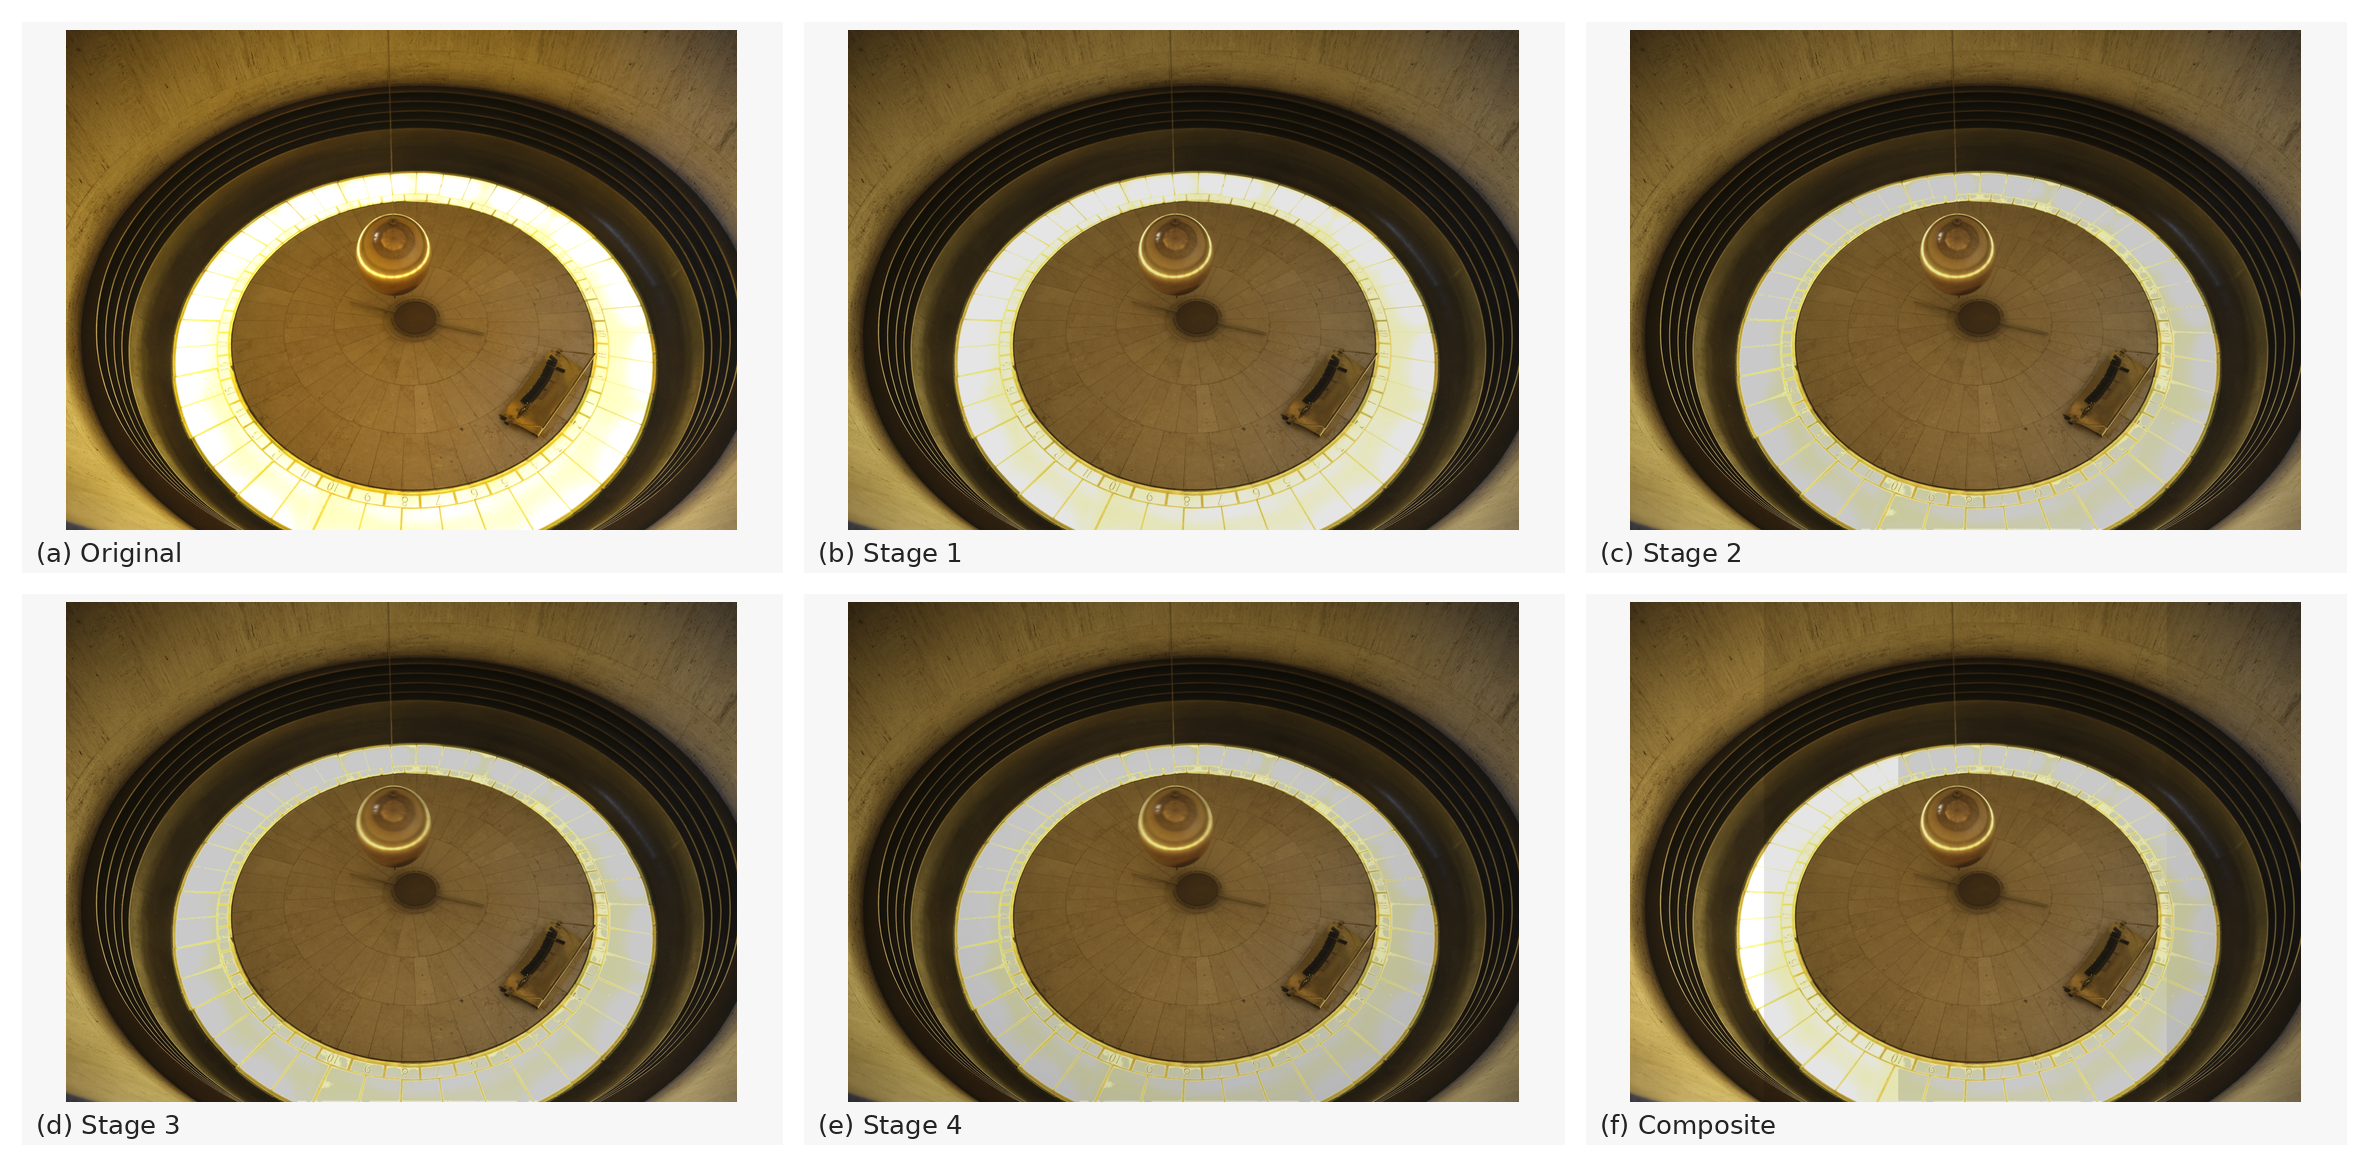
\includegraphics[width=.69\linewidth]{figures/case_1.png}

\caption{Pendulum case: (a) original; (b--e) four cumulative processing stages; (f) final composite. Operations involve overall exposure, local brightness of the light ring, sphere blur, and vignetting, in that order.}

\Description{Six-panel pendulum exposure, motion, and vignetting progression.}
\label{fig:case1}

\end{figure}

\FloatBarrier

\subsection{Vanishing Hand: The Shape of Forgetting}

In another test, the narrative stated, 'I want to forget her; I want her hand to disappear.' The system localized the hand and ring and gradually applied local whitening over three cumulative stages. White did not invisibly repair the background: it occupied the space formerly held by the hand and spread at its edge. Details retreated, yet the outline of absence remained. Aspen Mays's material 'erasure' and Kganye's silhouettes provide different references for disappearance; this work retains absence and reorganizes visibility by indicating an object and the space it once occupied.


\begin{figure}[htbp]

\centering

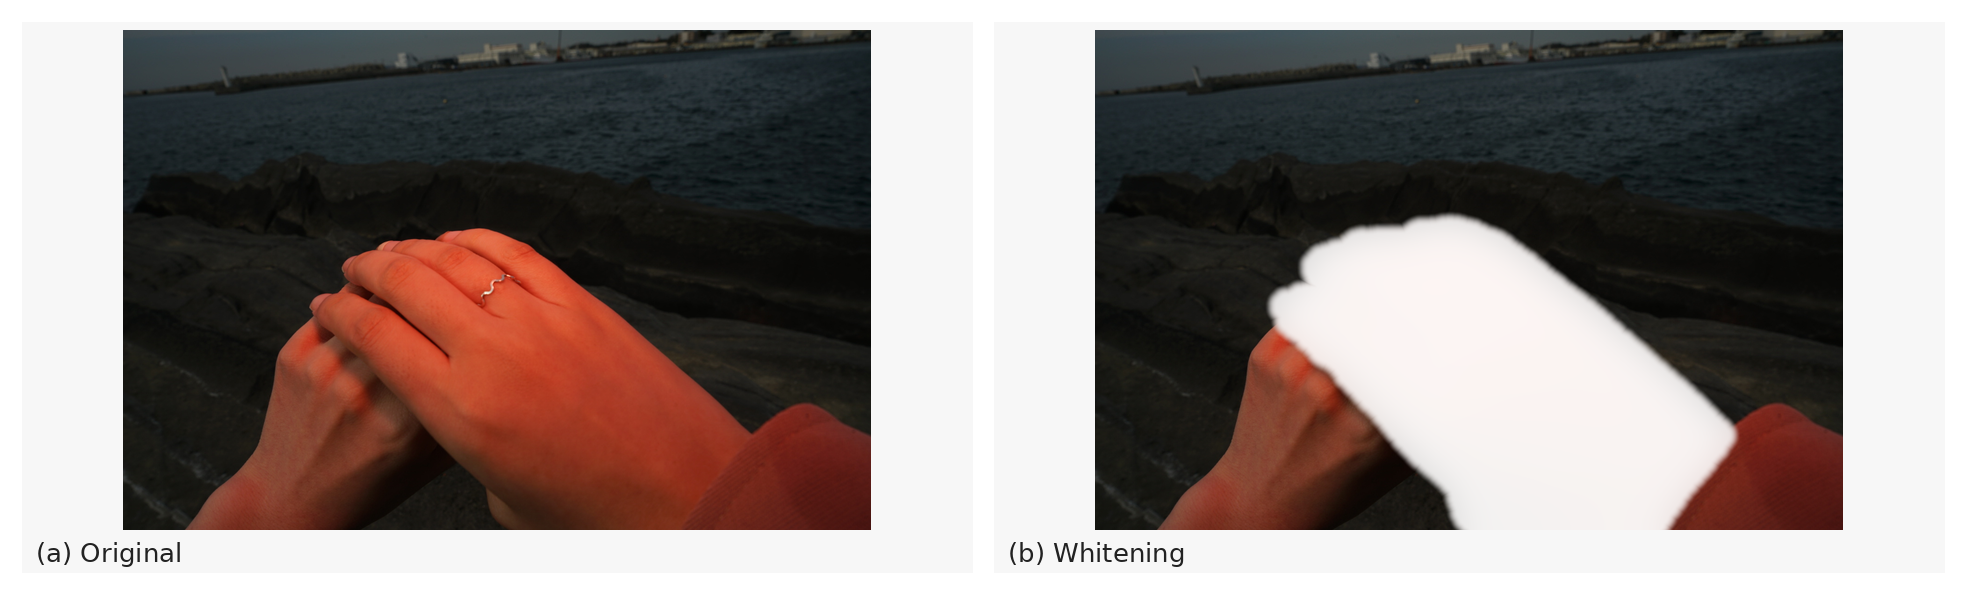
\includegraphics[width=.69\linewidth]{figures/case_2.png}

\caption{Vanishing-hand case: (a) original photograph; (b) local whitening result. The white region preserves the shape of absence rather than seamlessly regenerating the background.}

\Description{Two panel image showing original hands and whiteout treatment.}
\label{fig:case2}

\end{figure}

\FloatBarrier

\subsection{Adding an Index Finger: Touch Beyond the Frame}

A photograph of water, architecture, and a bird was accompanied by this narrative: 'I used my index finger to trace the outlines of these buildings at the time. I want to preserve that finger.' As no hand appeared in the original, a foreground gesture had to be added. In the test, generation was constrained by the entry edge, wrist connection, and intended fingertip target. The result is not the recovery of lost photographic evidence but a spatial possibility indicated by memory.


\begin{figure}[htbp]

\centering

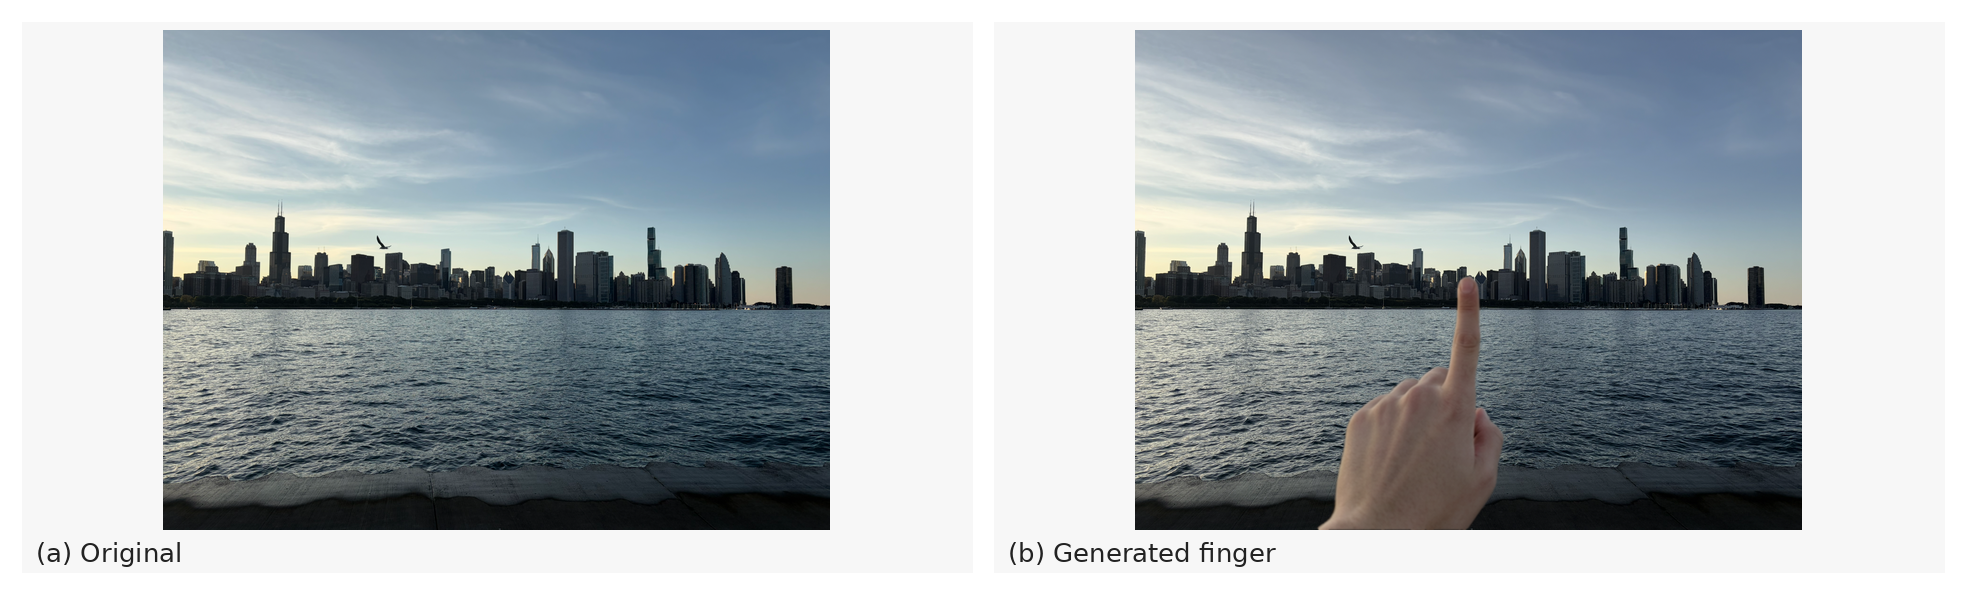
\includegraphics[width=.69\linewidth]{figures/case_3.png}

\caption{Adding an index finger: (a) original waterfront photograph; (b) a generated foreground finger guided by the narrative. The addition is a conjecture, not an image recorded at capture.}

\Description{Two panel image showing the original waterfront and generated index finger.}
\label{fig:case3}

\end{figure}

\FloatBarrier

\subsection{Forest: Spatial Rupture Beyond Framing}

The forest narrative reads: 'I cannot quite remember how the space looked then. I want the viewpoint to shift slightly to the side, with some misalignment and ruptures.' The process first generates a conjectural extension of the forest beyond the original frame, then inserts selected vertical and horizontal slices back into the photograph with horizontal stretching and hard-edged seams. Misaligned trunks, discontinuous terrain, and local repetition are permitted. Here, 'error' becomes an intended visual purpose, and the original record meets generated conjecture at visible seams.


\begin{figure}[htbp]

\centering

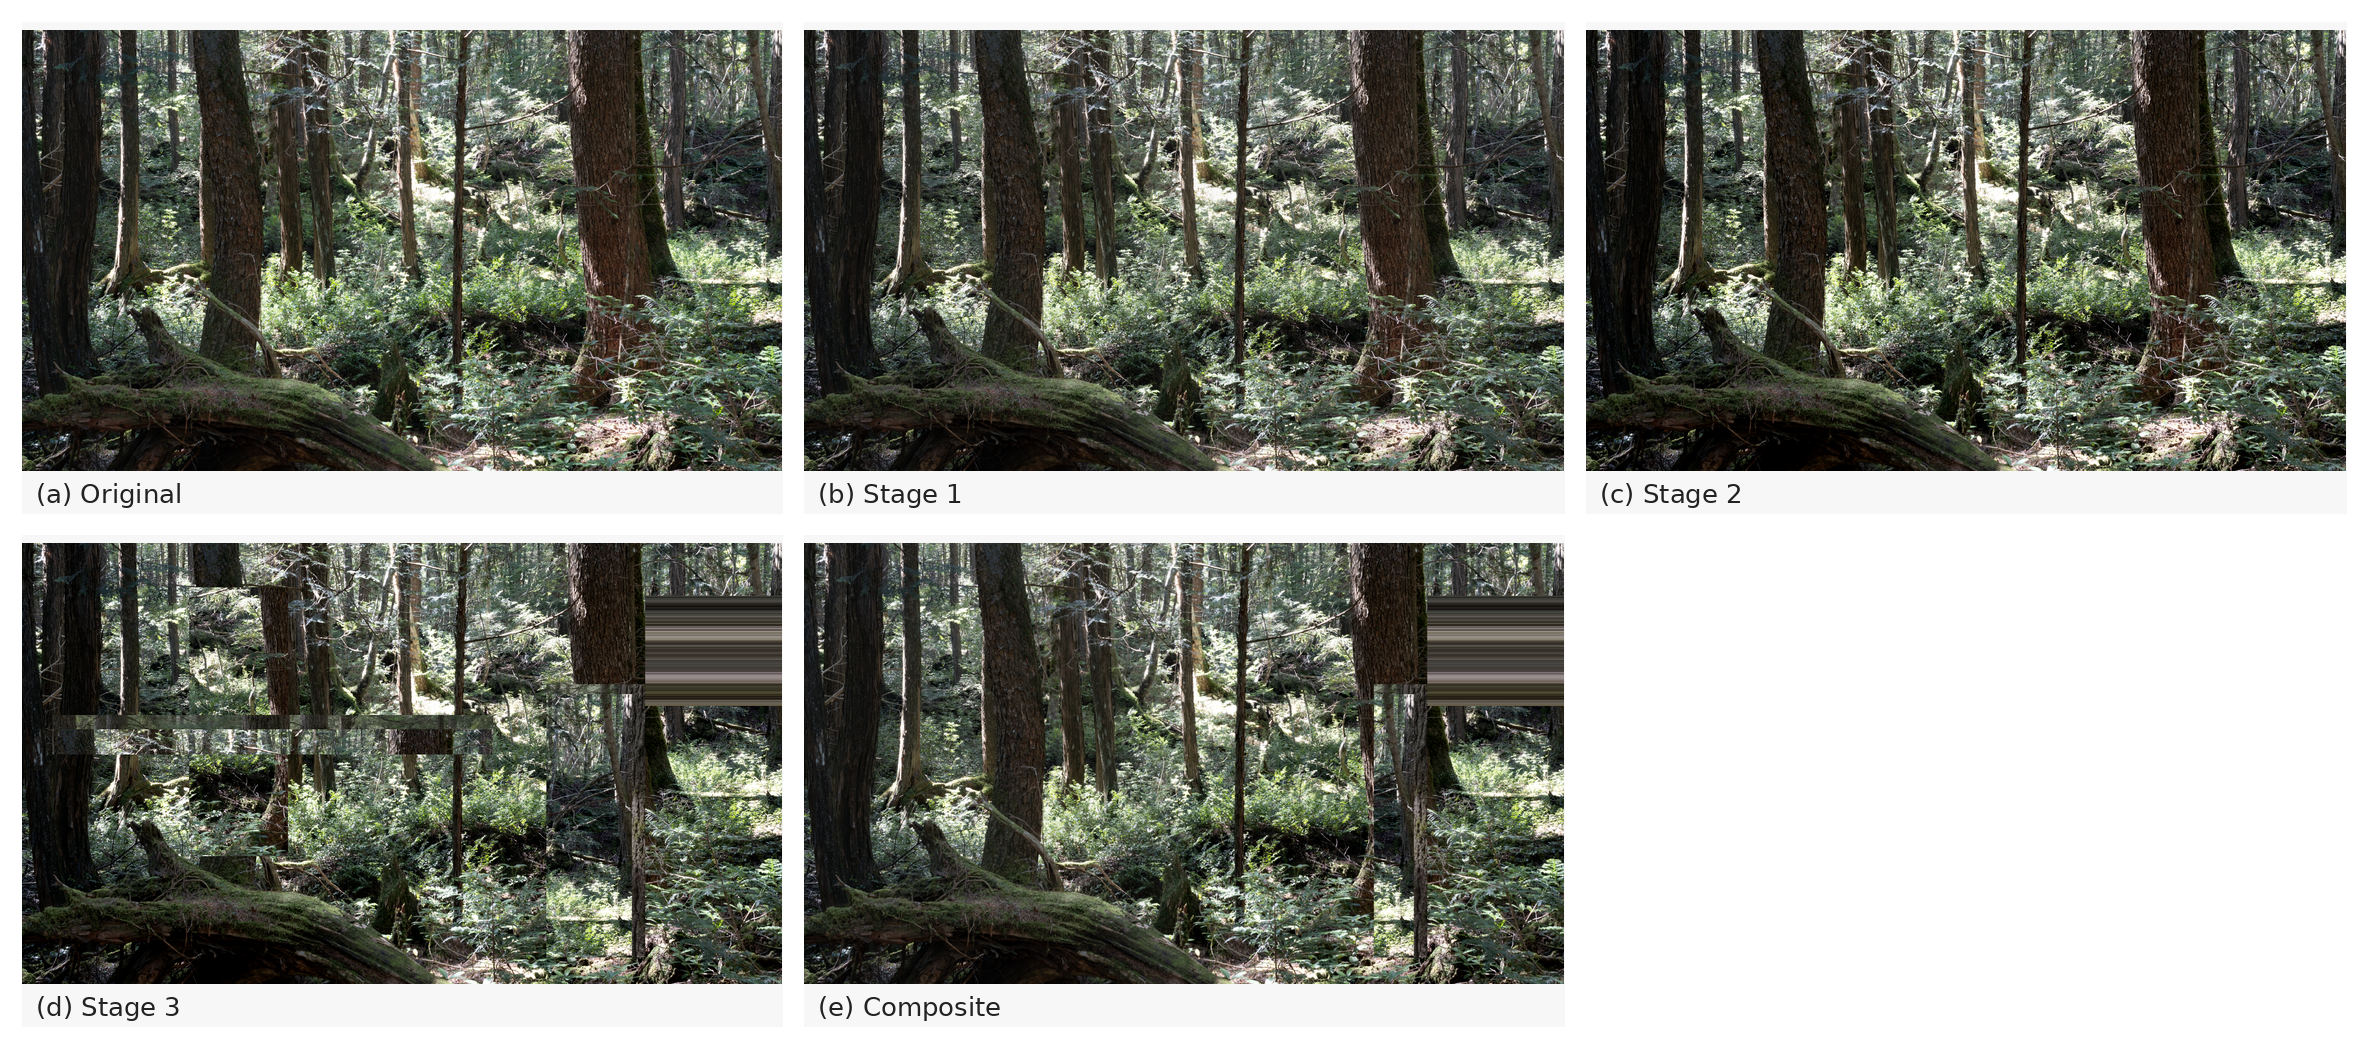
\includegraphics[width=.69\linewidth]{figures/case_4.png}

\caption{Forest spatial rupture: (a) original; (b--d) successive processing stages; (e) final cumulative composite. Slicing, hard seams, and local stretching reveal spatial discontinuity.}

\Description{Five-panel forest image showing original and cumulative fragments.}
\label{fig:case4}

\end{figure}

\FloatBarrier

\section{Discussion: How Incompleteness Becomes Poetic}

Alternative RAW renderings, concealment and defocus in artistic processing, and generative additions have different relations to photographic evidence: respectively, they are constrained by captured data, rework the viewing relation within an existing image, or create content absent at capture. Within one system, the same recollection might suggest whitening, a silhouette, or seamless removal. Poetry lies not in an individual algorithm but in choosing a relation between the visible and the invisible.


The method retains creative risks. Models may locate the wrong object; RAW effects depend on sensors and available file information; generation may introduce unintended details; vertical strips may hide the most important change in a stage. None of this proves that a memory has been faithfully restored, yet poetry may still emerge through the process. Recollection cannot be reconstructed as a precise image-processing path. Bergson's virtual memory is not an image cache, and a user's words are not a complete account of the past. Interpreting 'forgetting' as whitening and a sense of duration as motion blur always involves the artist's rules and the model's judgment.


'Re-development' therefore does not seek another true photograph hidden inside the camera, nor does it regard psychological memory as data directly readable by algorithms. Starting from photographic technology and photographic art, it rearranges the photograph's formation, loss, repair, and viewing. Completion is not simply abolished; rather, it shifts from a uniform and determinate final image to the question of how a sequence of changes is organized and seen.


\section{Conclusion}

This study has produced a prototype for photographic re-creation jointly driven by photographs and recollection narratives. Through semantic understanding, regional segmentation, constrained operations, and AI generation, the system translates words into successive changes applied to the previous image and composes corresponding strips from the original and cumulative stages into a final work.


Starting from the question 'Does a photograph have only one final form?', the research uses the image variability of ISP pipelines to organize traceable RAW re-development, non-generative methods of contemporary photographic art, and constrained AI additions into a layered artistic method. The pendulum reinterprets time; the whitened hand preserves the outline of forgetting; the added finger crosses the framing boundary; and the forest makes spatial conjecture and rupture visible.


Rather than finding the one image closest to the past, the work allows the original, the processing stages, and their provenance to constitute the artwork together. By gradual development, juxtaposition, and assembly, it makes no claim to reconstruct the true appearance of the past. It preserves how a photograph is modified, damaged, supplemented, and reorganized through narration in the present. Choices and transformations normally hidden by the final image become a photographic practice in which interpretation can be seen.


In this sense, the work orchestrates technical possibilities of camera imaging with human artistic interventions in photography. Through recollection, states normally corrected, hidden, or discarded re-enter the field of viewing, allowing photographic unfinishedness to become poetic expression. Bringing these changes from different sources into one production chain, it uses the intermediate states of the photographic medium to articulate recollection poetically, while leaving unresolved boundaries open for discussion.


\begin{thebibliography}{99}

\bibitem[Bergson(1991)]{ref66} Bergson, H. (1991). Matter and Memory (N. M. Paul \& W. S. Palmer, Trans.). Zone Books. (Original work published 1896).

\bibitem[Brown(2023)]{ref67} Brown, M. S. (2023). Color processing for digital cameras. In P. Green (Ed.), Fundamentals and Applications of Colour Engineering (pp. 81--98). Wiley. \url{https://doi.org/10.1002/9781119827214.ch5}

\bibitem[Domestic Data Streamers(2023)]{ref68} Domestic Data Streamers. (2023). Synthetic Memories [Art and research project]. \url{https://www.domesticstreamers.com/work/synthetic-memories/}

\bibitem[Flusser(2000)]{ref69} Flusser, V. (2000). Towards a Philosophy of Photography (A. Mathews, Trans.). Reaktion Books. (Original work published 1983).

\bibitem[Karaimer and Brown(2016)]{ref70} Karaimer, H. C., \& Brown, M. S. (2016). A software platform for manipulating the camera imaging pipeline. In Computer Vision -- ECCV 2016 (pp. 429--444). Springer. \url{https://doi.org/10.1007/978-3-319-46448-0_26}

\bibitem[Kitasono(1966)]{ref71} Kitasono, K. (1966). A note on plastic poetry. VOU, 104, 23. \url{https://www.kitasonokatue.com/new-page-4}

\bibitem[Kganye(2016)]{ref72} Kganye, L. (2016). Reconstruction of a Family [Artwork series]. Chazen Museum of Art collection record. \url{https://chazen.wisc.edu/collection/29751/re-palame-tereneng-e-fosahetseng-from-the/}

\bibitem[Mavropoulou(2021--2023)]{ref73} Mavropoulou, M. (2021--2023). Imagined Images [Art project]. \url{https://www.mariamavropoulou.com/imagined-images}

\bibitem[Mayer(1971)]{ref74} Mayer, B. (1971). Memory [Photography, text, and audio project; published by Siglio in 2020]. \url{https://sigliopress.com/readings/memory-mayer-history/}

\bibitem[Mays(2011)]{ref75} Mays, A. (2011). Punched Out Stars [Photographic series]. Museum of Contemporary Photography. \url{https://mocp.emuseum.com/objects/10613/punched-out-stars-10}

\bibitem[Müller-Pohle(1995--1998)]{ref76} Müller-Pohle, A. (1995--1998). Digital Scores (after Nicéphore Niépce) [Art project]. \url{https://muellerpohle.net/projects/digital-scores/}

\bibitem[Pataranutaporn et al.(2025)]{ref77} Pataranutaporn, P., Archiwaranguprok, C., Chan, S. W. T., Loftus, E., \& Maes, P. (2025). Synthetic human memories: AI-edited images and videos can implant false memories and distort recollection. In Proceedings of the 2025 CHI Conference on Human Factors in Computing Systems. \url{https://doi.org/10.1145/3706598.3713697}

\bibitem[rawpy(n.d.)]{ref78} rawpy. (n.d.). RawPy and Params API documentation [Online software documentation, accessed 24 November 2026]. \url{https://letmaik.github.io/rawpy/api/rawpy.RawPy.html} ; \url{https://letmaik.github.io/rawpy/api/rawpy.Params.html}

\bibitem[Ruff(2004--2007)]{ref79} Ruff, T. (2004--2007). jpegs [Photographic series]. Museum of Modern Art collection record. \url{https://www.moma.org/collection/works/149384}

\bibitem[Wade et al.(2002)]{ref80} Wade, K. A., Garry, M., Read, J. D., \& Lindsay, D. S. (2002). A picture is worth a thousand lies: Using false photographs to create false childhood memories. Psychonomic Bulletin \& Review, 9(3), 597--603. \url{https://doi.org/10.3758/BF03196318}

\bibitem[Zhang et al.(2024)]{ref81} Zhang, W., Cheng, L., \& Luo, J. (2024). ReCollection: Creating synthetic memories with AI in an interactive art installation. Proceedings of the ACM on Computer Graphics and Interactive Techniques, 7(4), Article 51, 1--10. \url{https://doi.org/10.1145/3664207}

\end{thebibliography}

\end{document}
